\section{Case study}\label{sec:case-study}
This section describes the practical experiment used to evaluate representations.

\subsection{Scenario and context}\label{subsec:scenario-and-context}
The purpose of the case study was to validate the previous evaluation in a more realistic scenario.
Additionally, this was an opportunity to assess the development experience using the representations.
These objectives were achieved by recreating a few screens of a fictional application modeled after Trello\furl{trello.com} -- a well-known Web application for creating Kanban-style lists.
The choice was motivated by its popularity and relative complexity.

The capabilities of the original application are broad and include detailed management of workspaces, users, and boards, as well as editing and managing content-rich cards.
It would not be reasonable to implement all these functionalities -- to keep the case study manageable, it was necessary to limit its scope.
The selected area to implement concerns the simple management of cards across two views and a single dialog window:
\begin{itemize}
    \item the first view allows viewing all boards the user has access to and navigating to a board (Figure~\ref{fig:3-4-boards-view})
    \item the second view allows viewing a particular board and its data -- name, columns, and cards (Figure~\ref{fig:3-4-board-view})
    \item the dialog window allows adding or editing a single card (Figure~\ref{fig:3-4-card-dialog})
\end{itemize}
Additionally, the representations should be able to represent two prominent components:
\begin{itemize}
    \item a column -- a board consists of multiple columns, each possibly containing multiple cards (Figure~\ref{fig:3-4-column-component})
    \item a card -- contains information about a task (Figure~\ref{fig:3-4-card-component})
\end{itemize}

The navigation map in Figure~\ref{fig:3-4-navigation-map} sums up all the application screens and their relationships.
This setup covers all four CRUD operations, making the case study representative of real-life applications.
The management of boards and columns within a board was omitted to keep the example as small as possible;
for the same reason, the interface was only implemented in a mobile version -- it is considered a good practice to design applications and websites using the \enquote{mobile first} principle\furl{https://developer.mozilla.org/en-US/docs/Web/Progressive_web_apps/Responsive/Mobile_first}.

\begin{figure}[tbh]
    \centering
    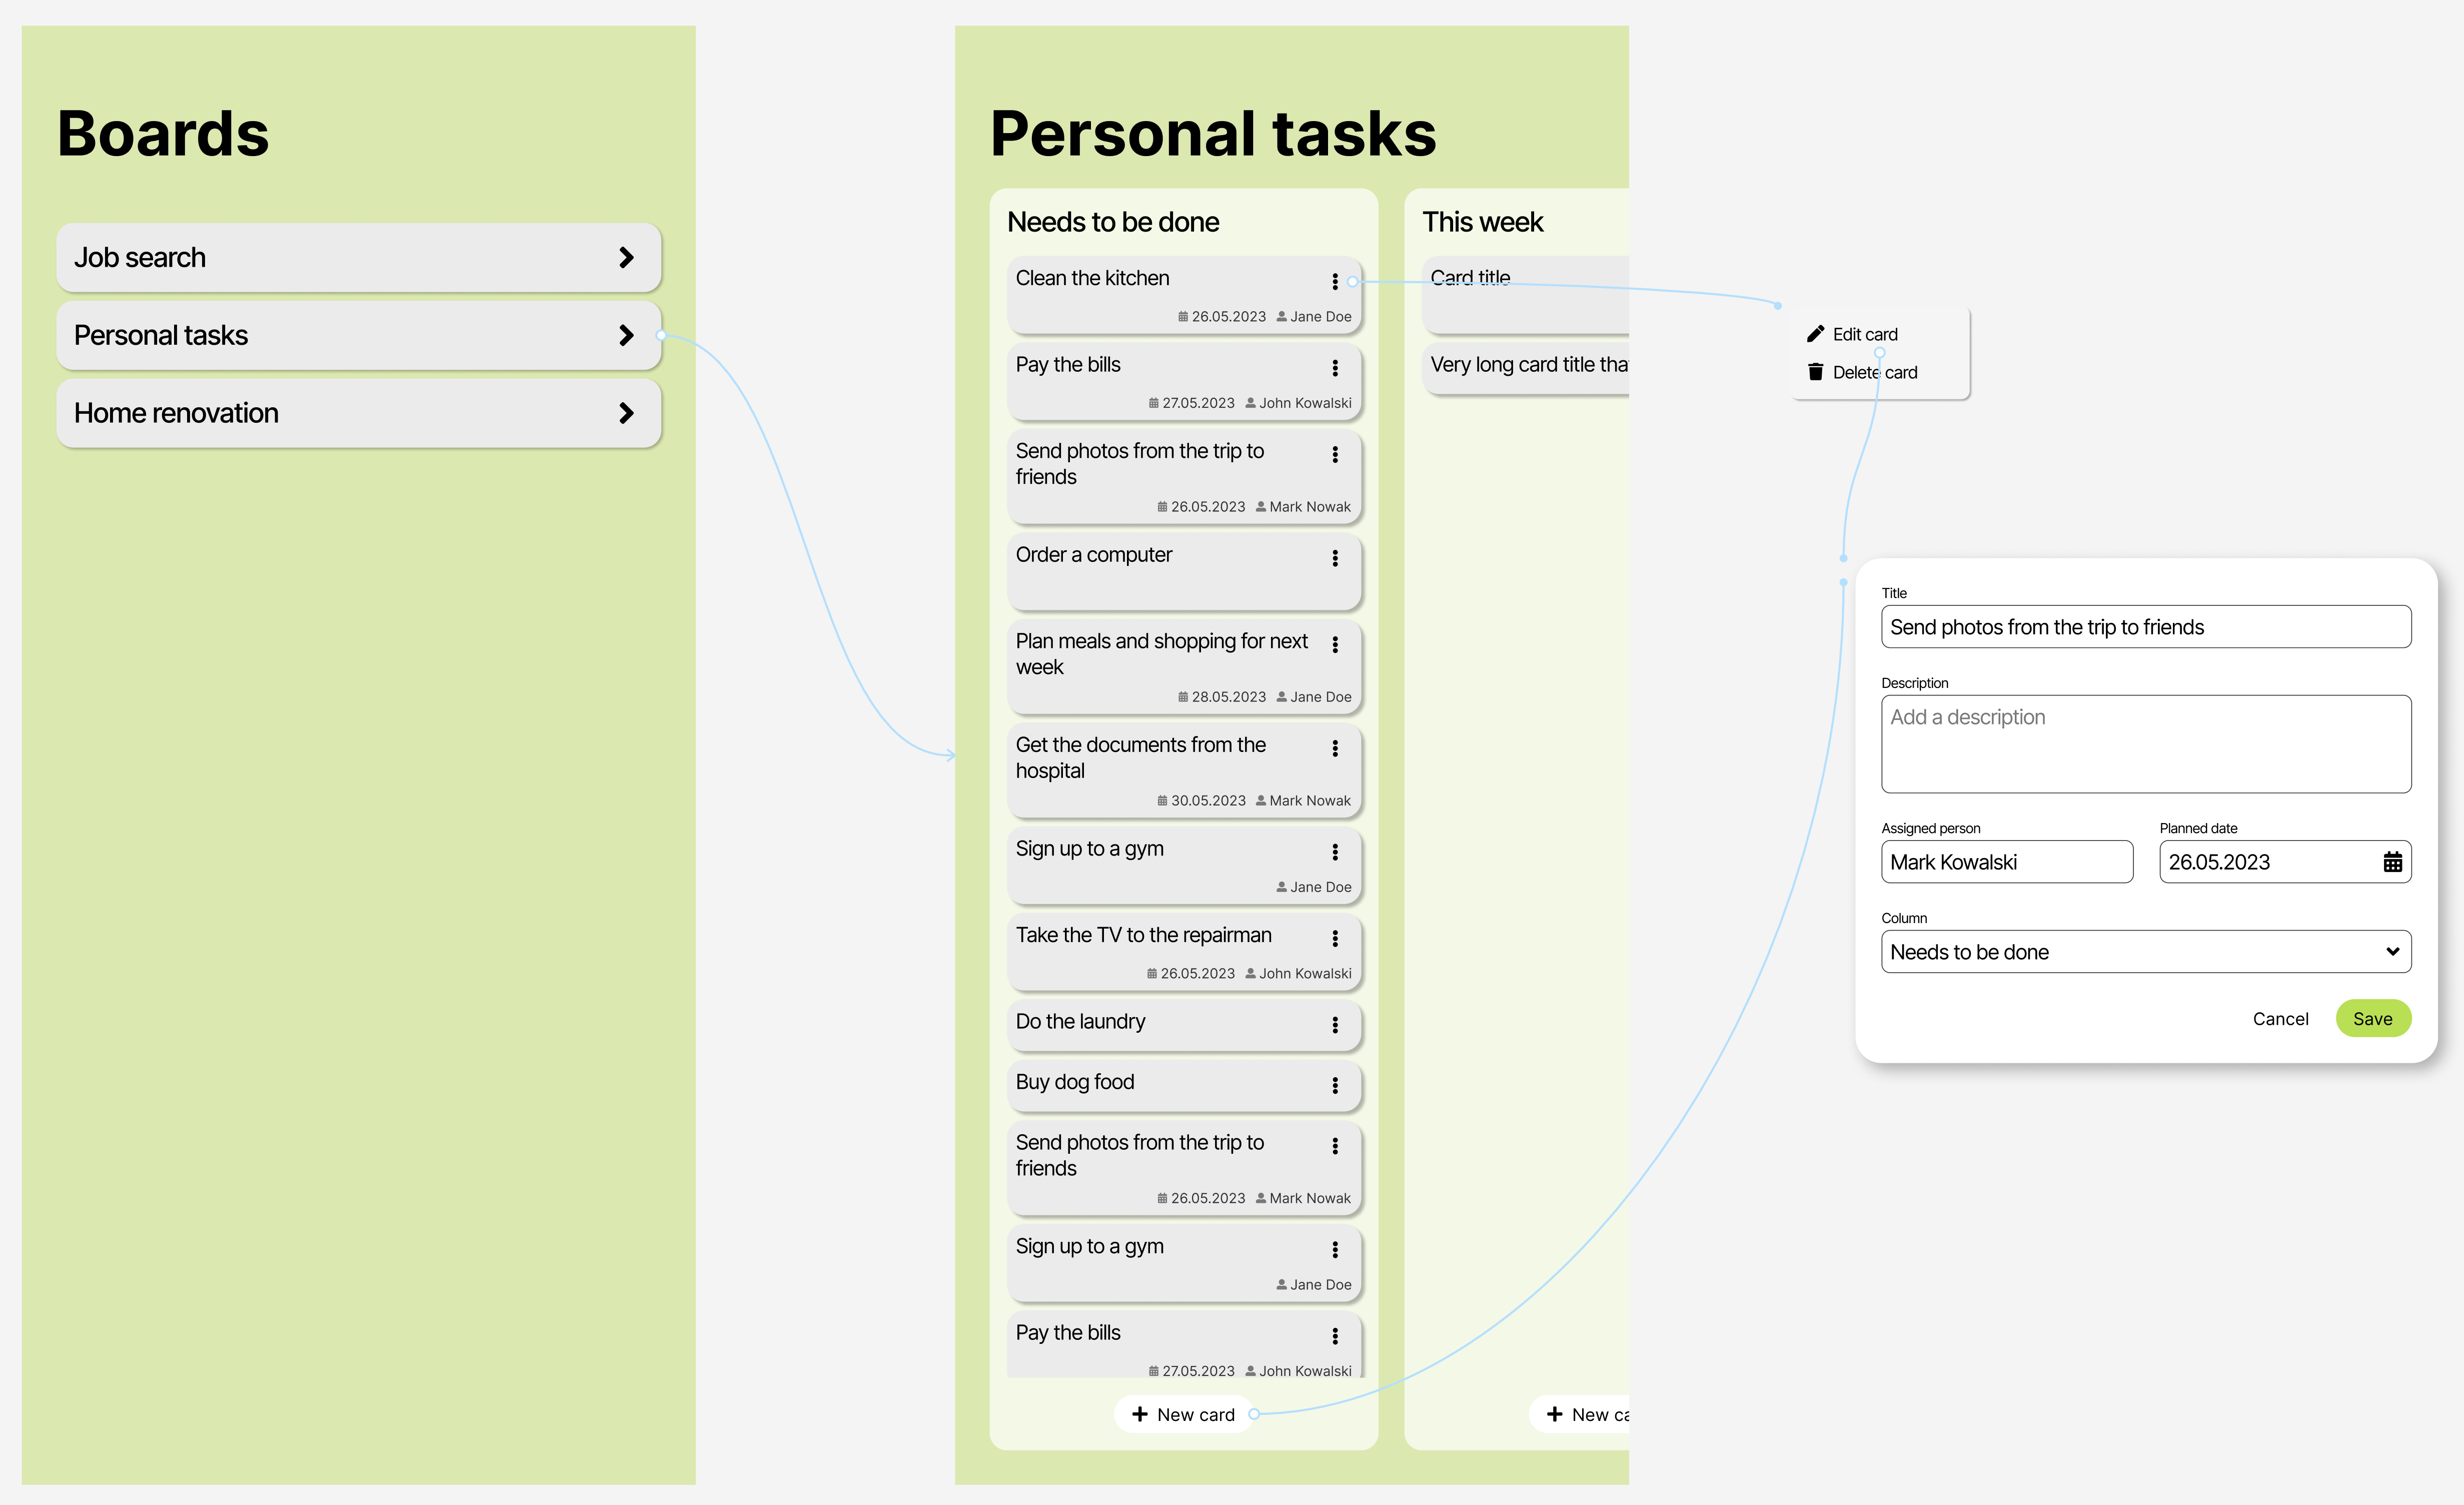
\includegraphics[width=\textwidth]{3-research-methodology/nav-map}
    \caption{Navigation map of application views}
    \label{fig:3-4-navigation-map}
\end{figure}

\subsection{Scoring of representations}\label{subsec:scoring-of-representations2}

The subsequent sections provide a description of functionalities that the representations were expected to implement;
Table~\ref{tab:case-study-requirements} summarizes them across five sections -- each corresponding to an implementation area described beforehand.
This time, the requirements were not prescriptive and did not specify how exactly they should be implemented.
This was meant to produce a more realistic evaluation.
To reflect this freedom of implementation, the evaluation of requirements included a score for partial fulfillment, not only a binary score.

Each requirement RX.Y is assigned a score $R_{\text{X.Y}}$ based on the Equation~\ref{eq:3-4-requirement-scoring}:
\begin{equation}
    R_{\text{X.Y}} =
    \begin{dcases}
        0   & \text{if the requirement is not satisfied}\\
        0.5 & \text{if the requirement is partially satisfied}\\
        1   & \text{if the requirement is satisfied}
    \end{dcases}
    \label{eq:3-4-requirement-scoring}
\end{equation}

The score $R_{\text{X}}$ for each area RX is the average score of all the requirements for the area (Equation~\ref{eq:3-4-area-scoring}).
The total score $T_{\text{requirements}}$ for the whole representation is calculated similarly (Equation~\ref{eq:3-4-representation-scoring}).

\begin{equation}
    R_{\text{X}} = \frac{\sum_{i=1}^{n} R_{\text{X.$i$}}}{n}
    \label{eq:3-4-area-scoring}
\end{equation}

\begin{equation}
    T_{\text{requirements}} = \frac{\sum_{i=1}^{5} R_i}{5}
    \label{eq:3-4-representation-scoring}
\end{equation}

\begin{longtblr}[
    caption = {Requirements for parts of the interface developed in the case study},
    label = {tab:case-study-requirements},
]{
    colspec = {cX[3,c]c},
    rowhead = 1,
    rows = {m},
}
    \hline[1pt]
    \textbf{Number} & \textbf{Requirement name}                                                       & \textbf{Related criteria}                          \\*
    \hline[1pt]
    \textbf{R1}     & \textbf{Boards view}                                                            & \textemdash                                        \\*
    R1.1            & view title has a bold, very large font                                          & D7.1, D7.2                                         \\*
    R1.2            & boards are loaded when the view is opened                                       & \textbf{B6}, B4.7                                  \\*
    R1.3            & bords are displayed                                                             & B8.2.2, \textbf{B9}                                \\*
    R1.4            & clicking on a board navigates to the selected board                             & \textbf{B1}, \textit{B2.1.3}, B4.1                 \\
    \hline
    \textbf{R2}     & \textbf{Board view}                                                             & \textemdash                                        \\*
    R2.1            & columns (and cards) are loaded when the view is opened                          & \textbf{B6}, B4.7                                  \\*
    R2.2            & columns are displayed in a horizontal layout                                    & D1.1                                               \\*
    R2.3            & columns can be scrolled when they don't fit on the screen                       & \textbf{D3}                                        \\
    \hline
    \textbf{R3}     & \textbf{Column component}                                                       & \textemdash                                        \\*
    R3.1            & container has some padding                                                      & D6.1                                               \\*
    R3.2            & title is displayed at the top (and doesn't move when scrolling cards)           & \textbf{D4}                                        \\*
    R3.3            & cards displayed in a column, slightly separated from one another                & D1.1, D1.2                                         \\*
    R3.4            & cards can be scrolled when they don't fit                                       & \textbf{D3}                                        \\*
    R3.5            & new card button is displayed at the bottom (and doesn't move when scrolling)    & C6.1, \textbf{D4}                                  \\*
    R3.6            & new card button is slightly separated from the cards and is centered            & D6.1, D6.2                                         \\*
    R3.7            & new card button has a plus icon                                                 & \textbf{A4}, C2.1                                  \\*
    R3.8            & new card button opens a card dialog without data when clicked                   & \textbf{B1}, \textit{B2.1.3}, B4.3                 \\
    \hline
    \textbf{R4}     & \textbf{Card component}                                                         & \textemdash                                        \\*
    R4.1            & card button is displayed in the top right corner of the card                    & C6.1, \textbf{D4}                                  \\*
    R4.2            & card button opens a context menu when clicked                                   & \textbf{B1}, \textit{B2.1.3}, B4.7, C1.6           \\*
    R4.3            & editing card item opens a dialog with card data when clicked                    & \textit{B2.1.3}, B4.3                              \\*
    R4.4            & delete card item deletes the card from the column when clicked                  & \textit{B2.1.3}, B4.6, B4.7, B4.8                  \\*
    R4.5            & delete card item calls an appropriate service when clicked                      & \textit{B2.1.3}, \textbf{B6}                       \\*
    R4.6            & card indicators are written in grey text                                        & D7.6                                               \\*
    R4.7            & card indicators display icons                                                   & \textbf{A4}, C2.1                                  \\
    \hline
    \textbf{R5}     & \textbf{Card dialog}                                                            & \textemdash                                        \\*
    R5.1            & empty inputs have placeholders                                                  & \textit{C5.2.2}                                    \\*
    R5.2            & title field is required                                                         & \textit{C5.1.2}                                    \\*
    R5.3            & title field displays a custom error message when the input is empty             & B5.6                                               \\*
    R5.4            & card description field is a multi-row input                                     & \textit{C4.3.12}                                   \\*
    R5.5            & assigned person and planned date fields are shorter and displayed in single row & D1.2, D3.2                                         \\*
    R5.6            & planned date field is a date input                                              & \textit{C4.3.5}                                    \\*
    R5.7            & column field allows selecting from all columns in the board                     & C4.7                                               \\*
    R5.8            & cancel button discards the changes                                              & B1, \textit{B2.1.3}, \textbf{B3}, B4.4             \\*
    R5.9            & save button adds or updates the card                                            & B1, \textit{B2.1.3}, \textbf{B3}, B4.6, B4.7, B4.8 \\*
    R5.10           & save button calls a service                                                     & B1, \textit{B2.1.3}, \textbf{B3}, \textbf{B6}      \\*
    R5.11           & save button is not active if the title is not provided                          & B5, \textit{B8.2.1}, \textit{C5.2.1}, C6.1         \\
    \hline[1pt]
\end{longtblr}

\subsubsection{The boards' view}

\begin{figure}
    \centering
    \begin{minipage}{0.45\textwidth}
        \centering
        
\includegraphics[height=0.4\textheight]{./3-research-methodology/boards-view}
        \caption{An example design of a boards view.}
        \label{fig:3-4-boards-view}
    \end{minipage}
    \hfill
    \begin{minipage}{0.45\textwidth}
        \centering
        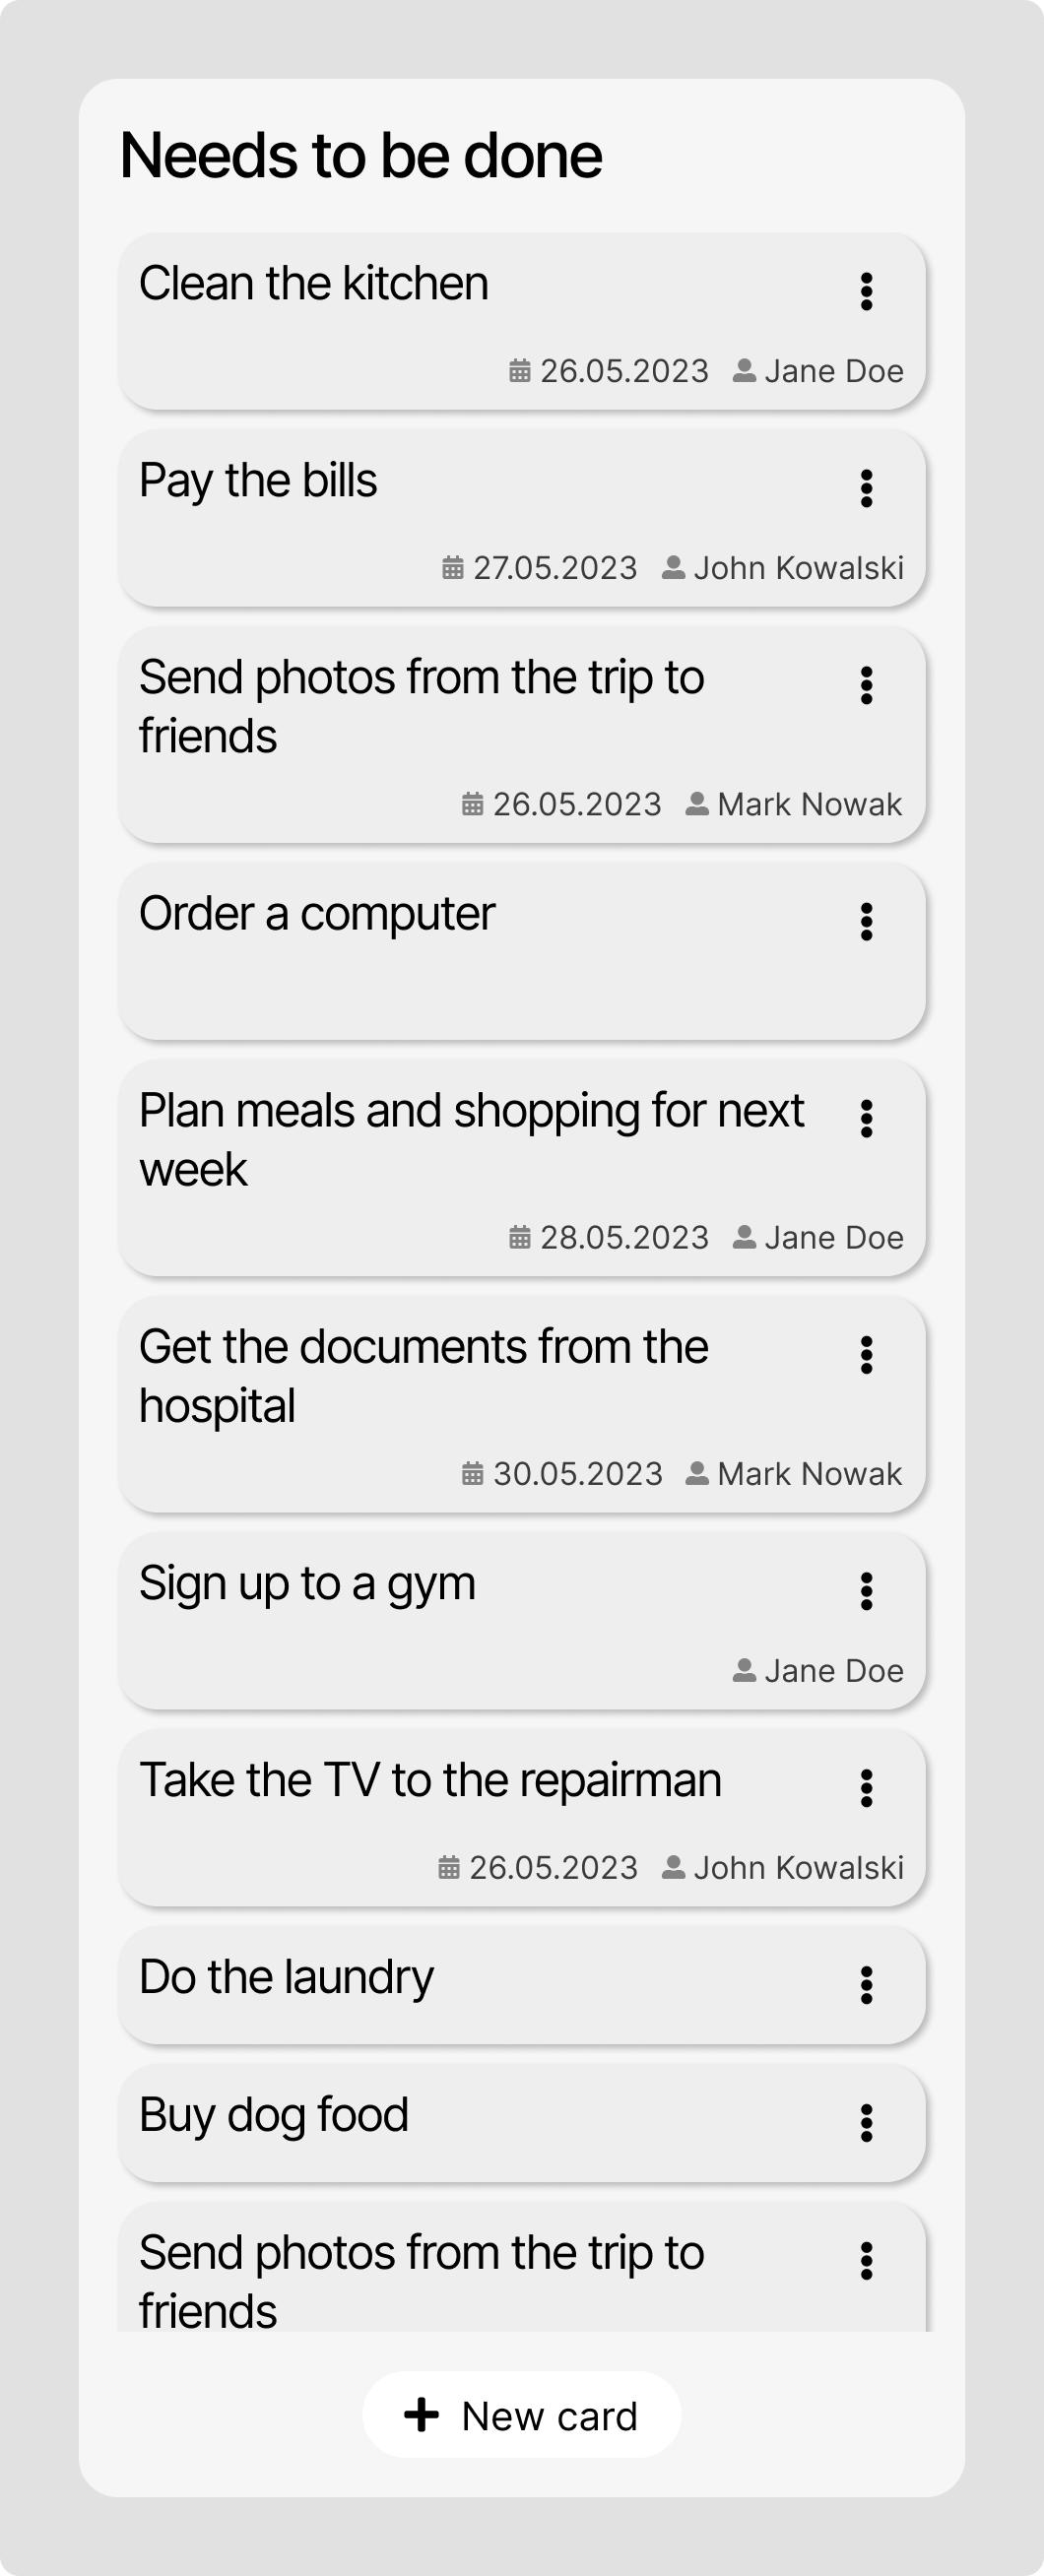
\includegraphics[height=0.4\textheight]{./3-research-methodology/column-component}
        \caption{An example design of a column component.}
        \label{fig:3-4-column-component}
    \end{minipage}
\end{figure}

The boards' view (presented in Figure~\ref{fig:3-4-boards-view}) is the application entry point.
In this case study, it only consists of the header and the list of boards the user can access.
The user can navigate to each board by clicking on a card with its name.

\subsubsection{The board view}
The board view, presented in figure~\ref{fig:3-4-board-view-expanded}, consists of a title and multiple columns.
Only the part with the green background is visible to the user;
the rest of the columns need to be scrolled to the view to be visible.

\begin{figure}
    \centering
    \begin{subfigure}[m]{0.6\textwidth}
        \centering
        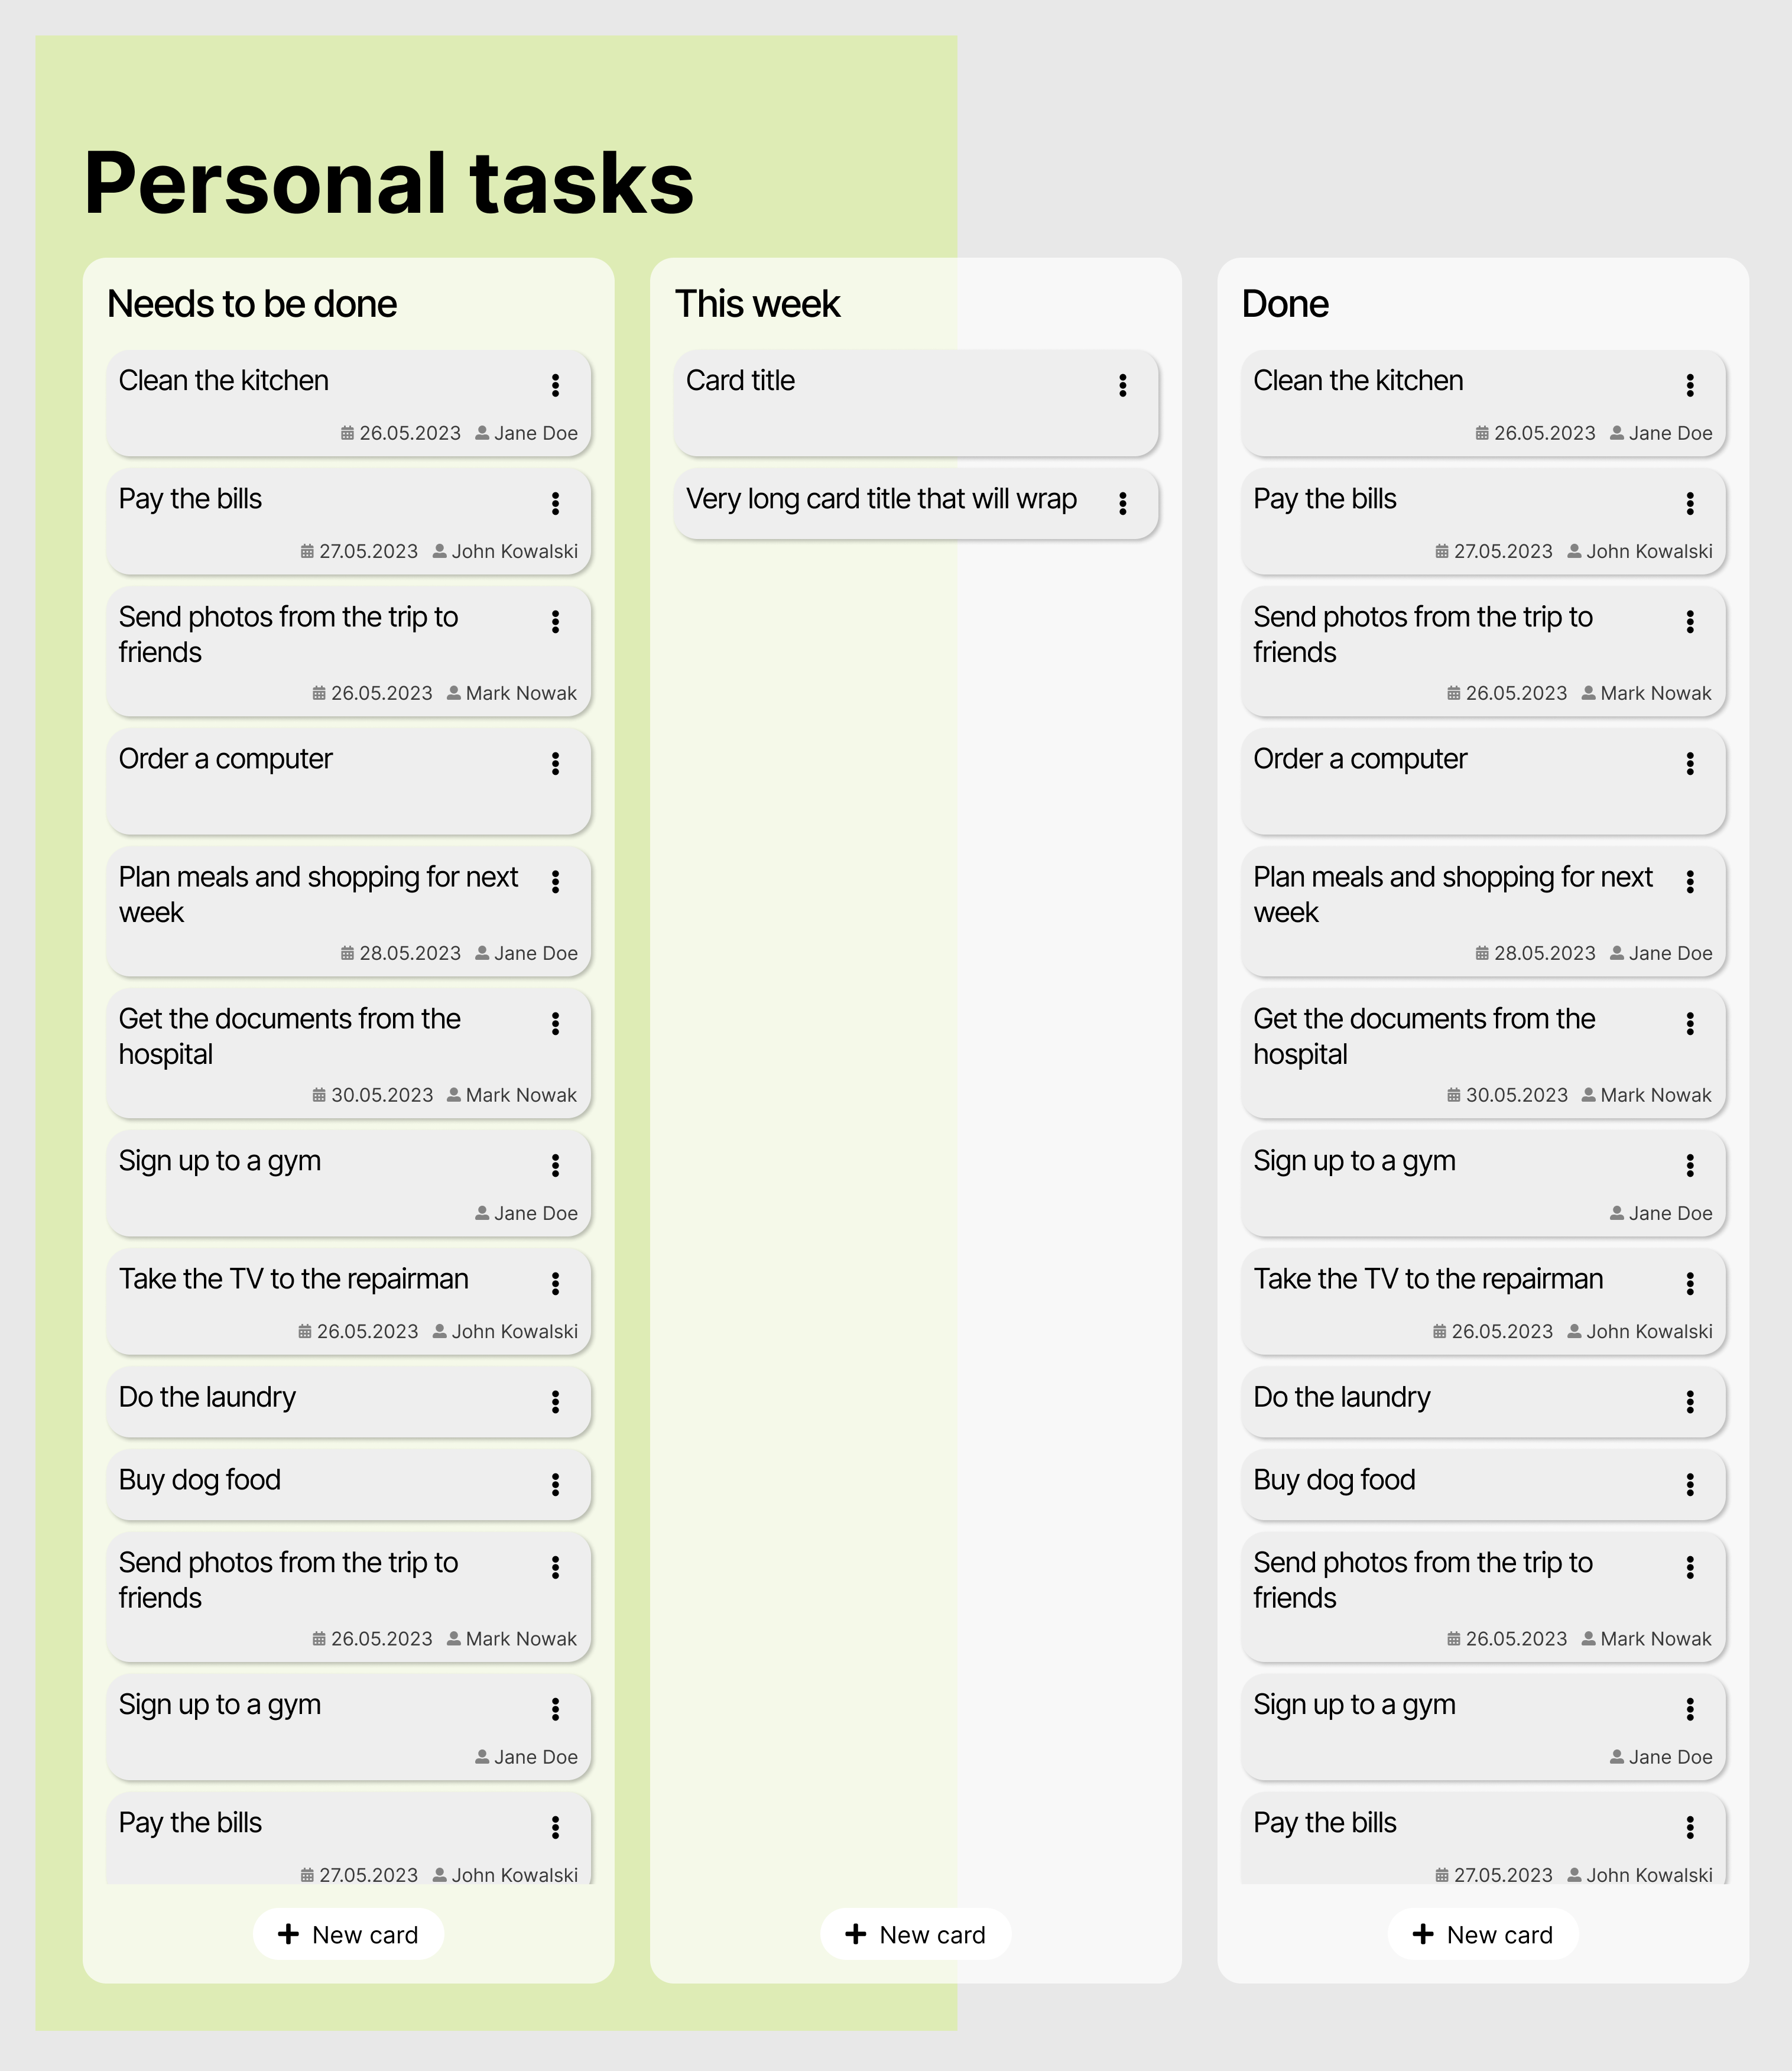
\includegraphics[height=0.4\textheight]{./3-research-methodology/board-view}
        \caption{Board view with overflowing content}
        \label{fig:3-4-board-view-expanded}
    \end{subfigure}
    \hfill
    \begin{subfigure}[m]{0.35\textwidth}
        \centering
        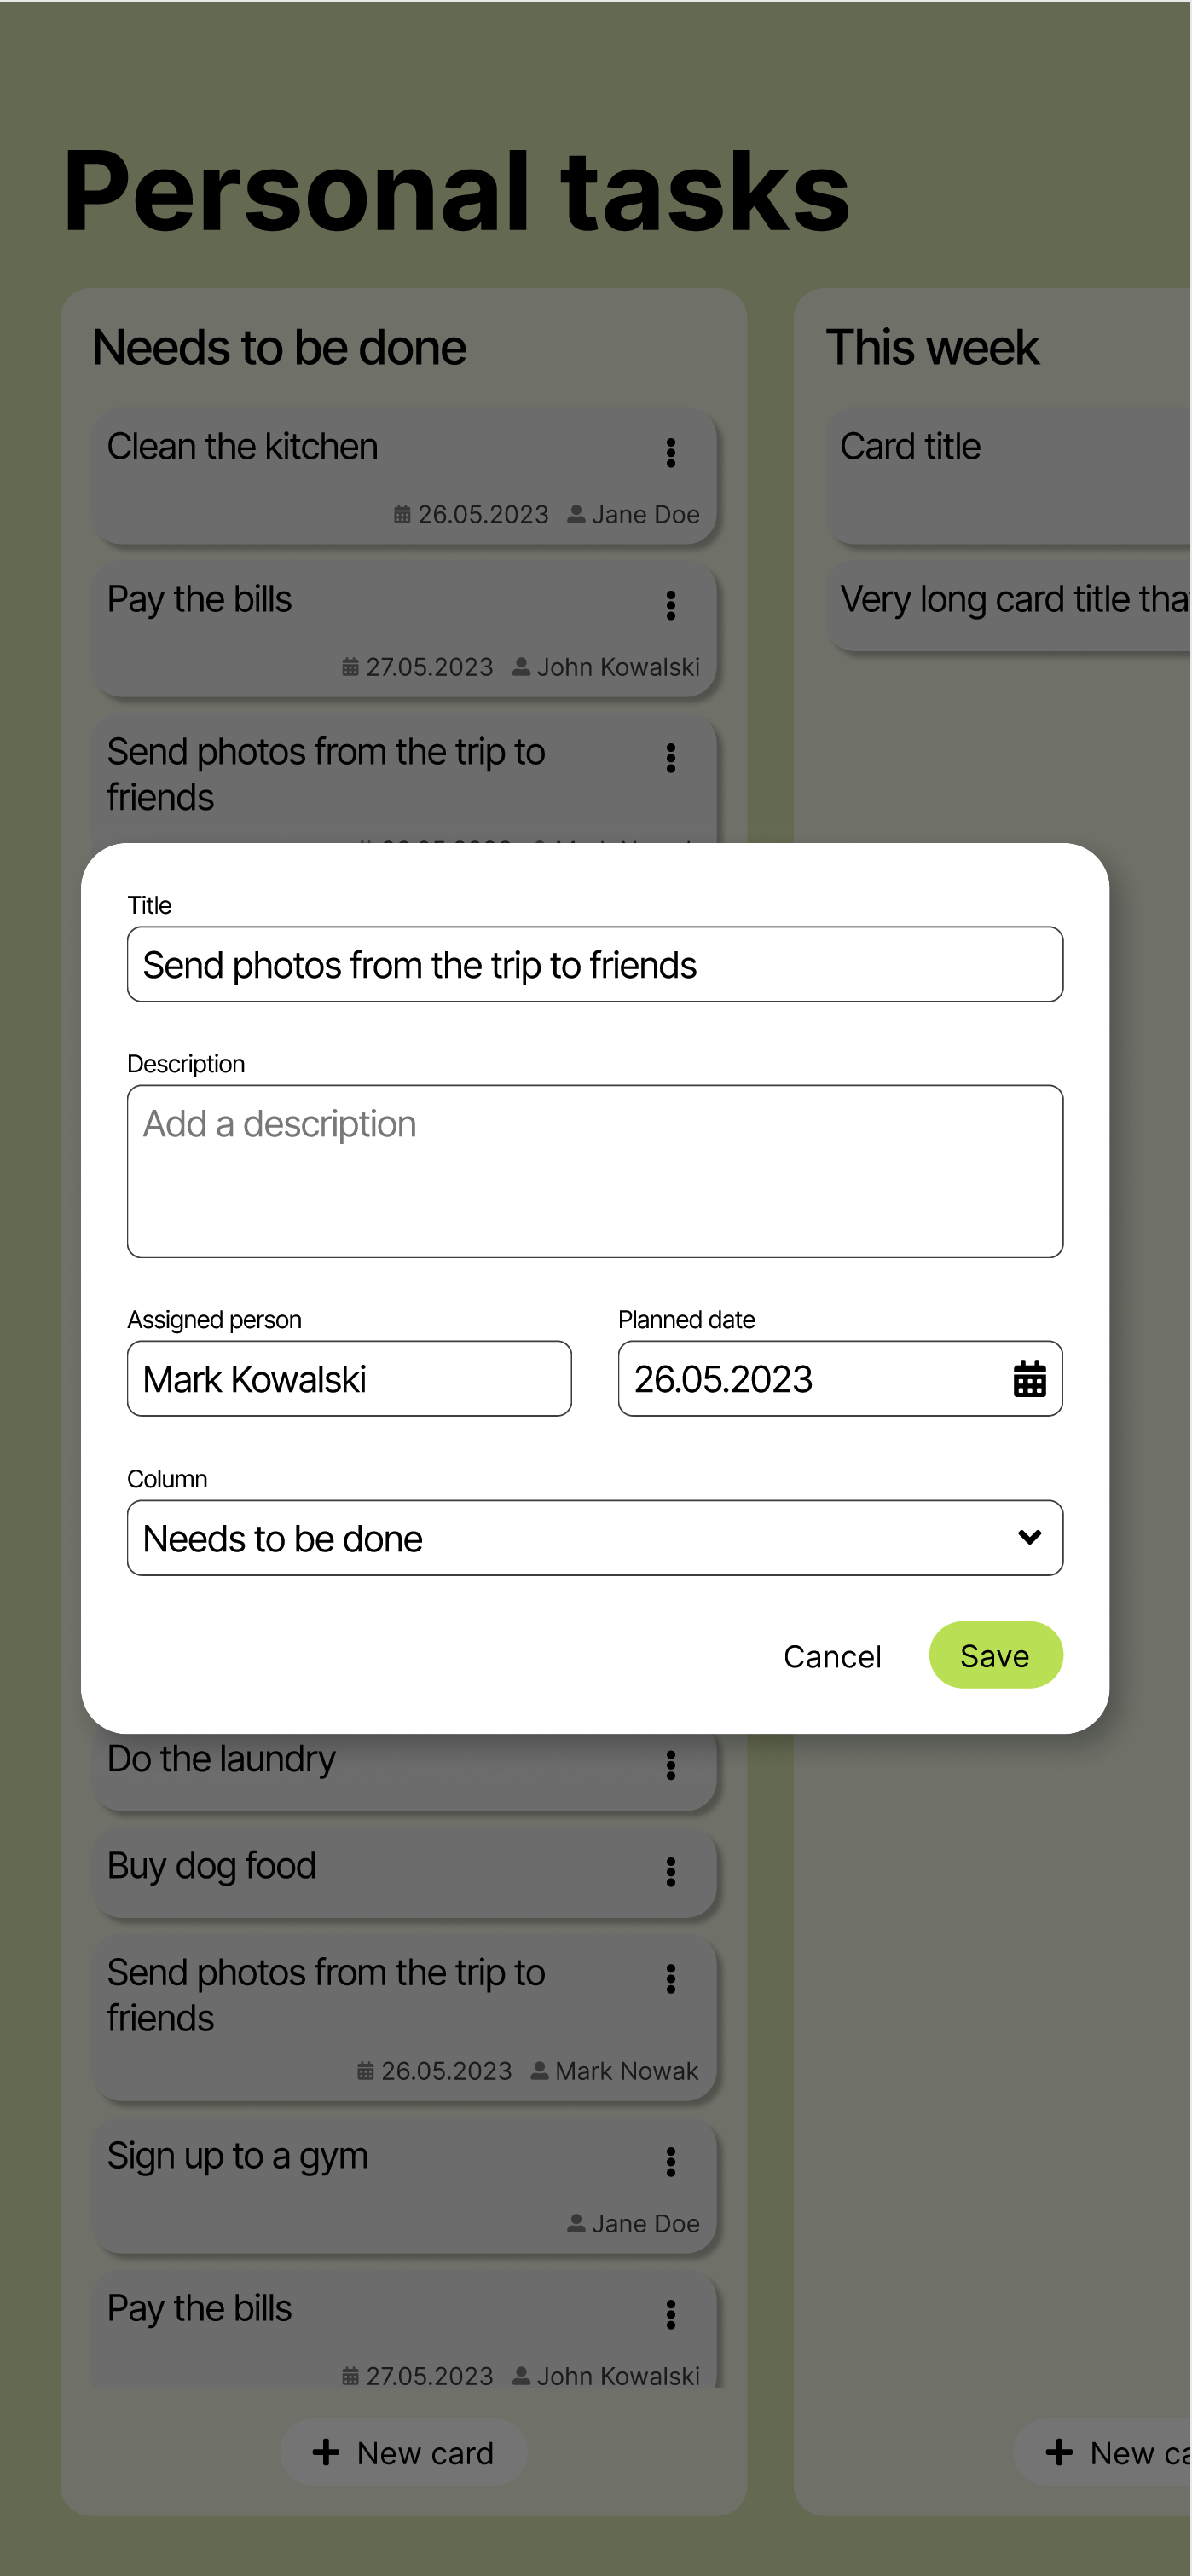
\includegraphics[height=0.4\textheight]{./3-research-methodology/board-view-with-dialog}
        \caption{Board view with the card editing dialog}
        \label{fig:3-4-board-view-with-dialog}
    \end{subfigure}
    \caption{An example design of a board view.}
    \label{fig:3-4-board-view}
\end{figure}

\subsubsection{The column component}
The column component, presented in figure~\ref{fig:3-4-column-component}, consists of three parts: a title at the top, a set of cards, and a button for adding new cards at the bottom.
The button opens a dialog window with a form for providing data about the card.
The upper and lower parts are \enquote{stuck} to the edges of the container: the title is always on the top of the container;
the button is at the bottom, and cards take the rest of the space of the container, scrolling if they cannot fit.

\subsubsection{The card component}
Figure~\ref{fig:3-4-card-component} depicts a card component, consisting of a title and various indicators (short texts with an icon) -- that unobtrusively signal information about a list item.
In the top-right corner of the card, there is a button that opens a context menu with two items: one that allows for editing a card (by opening a dialog) and the other that deletes a card.

\begin{figure}
    \centering
    \begin{subfigure}[m]{0.45\textwidth}
        \centering
        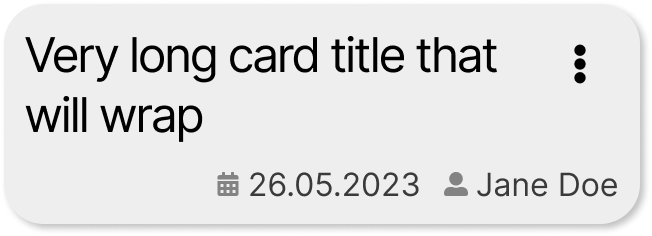
\includegraphics[width=\textwidth]{./3-research-methodology/card-component}
        \caption{Card component in a default state}
        \label{fig:3-4-card-component-plain}
    \end{subfigure}
    \hfill
    \begin{subfigure}[m]{0.45\textwidth}
        \centering
        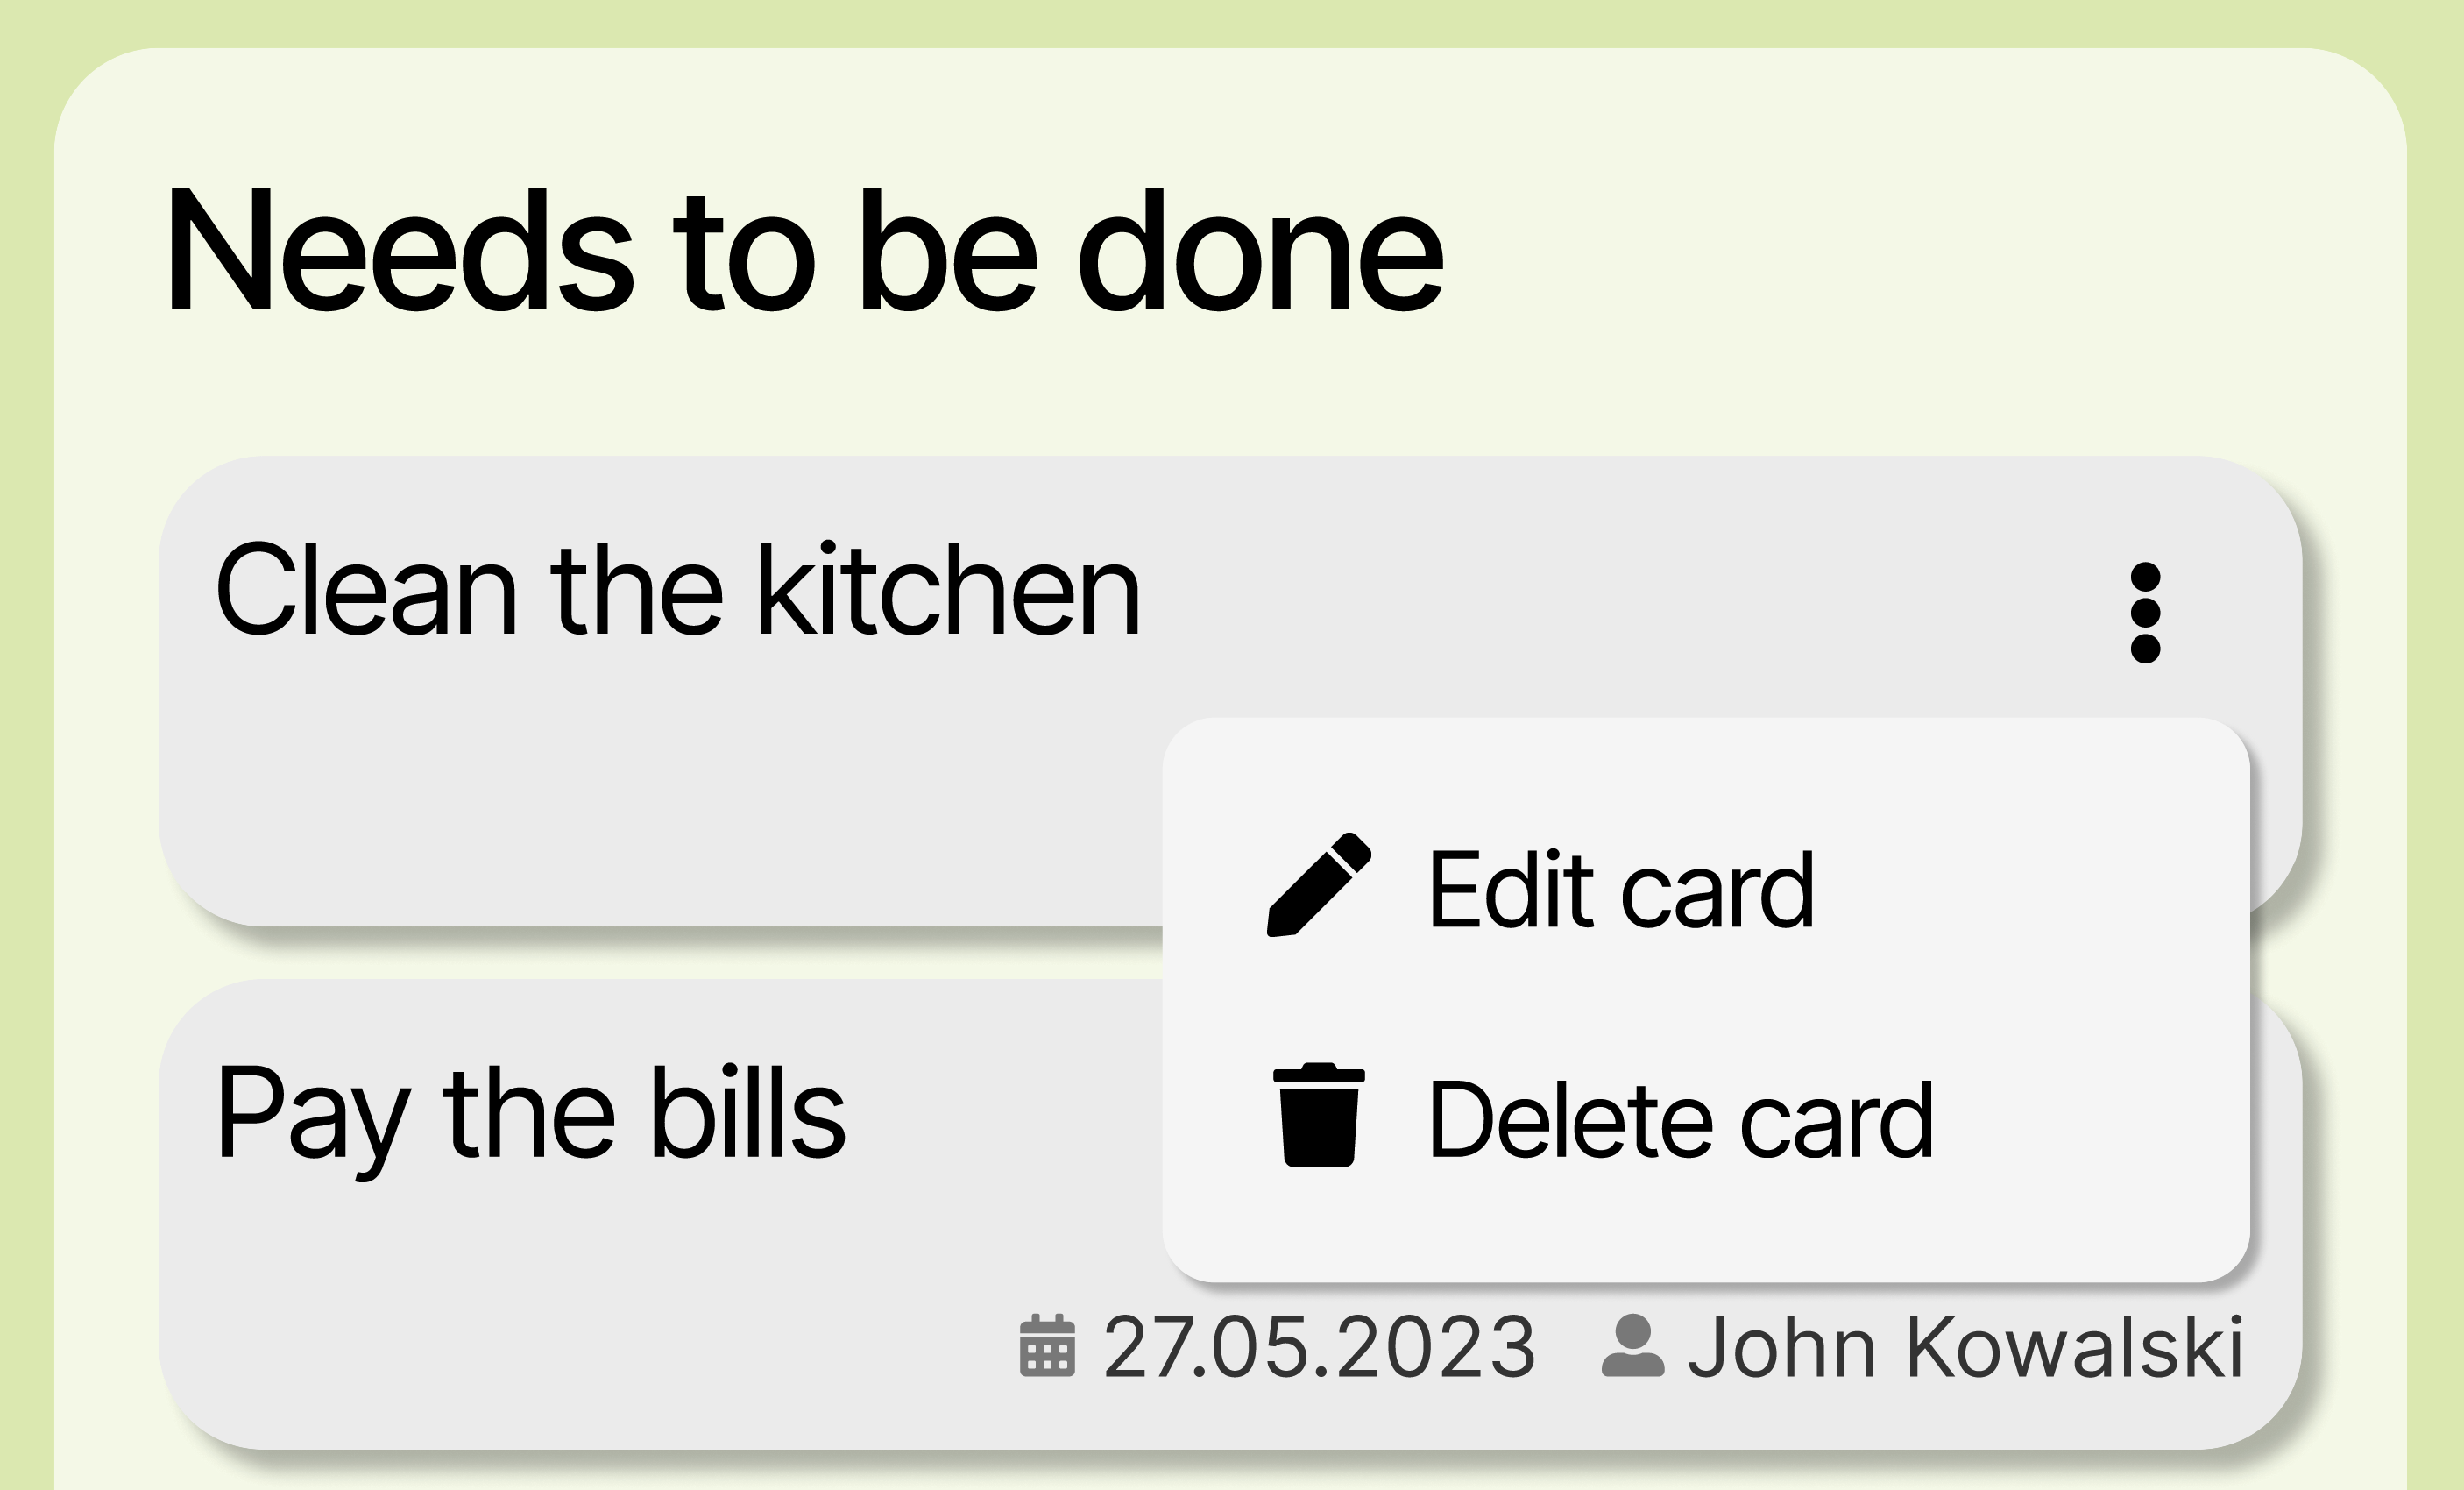
\includegraphics[width=\textwidth]{./3-research-methodology/card-component-with-menu}
        \caption{Card component with menu opened.}
        \label{fig:3-4-card-component-with-menu}
    \end{subfigure}
    \caption{An example design of a card component}
    \label{fig:3-4-card-component}
\end{figure}

\subsubsection{The card editing dialog}
The dialog is presented in Figures~\ref{fig:3-4-card-dialog} (on its own) and~\ref{fig:3-4-board-view-with-dialog} (in the context of a board view).
It is essentially a simple form -- a user can use it to provide information about a card: a title, a description, a person responsible for the card, a date, and the column.
Two buttons are placed at the bottom of the view -- one for discarding the edits and the other for saving them.
Only the title field is explicitly validated as a mandatory field.
The column field is also required but does not need validation, as its value is selected from a set of given values (columns).
The rest of the fields are optional.

\begin{figure}
    \centering
    \begin{subfigure}[m]{0.45\textwidth}
        \centering
        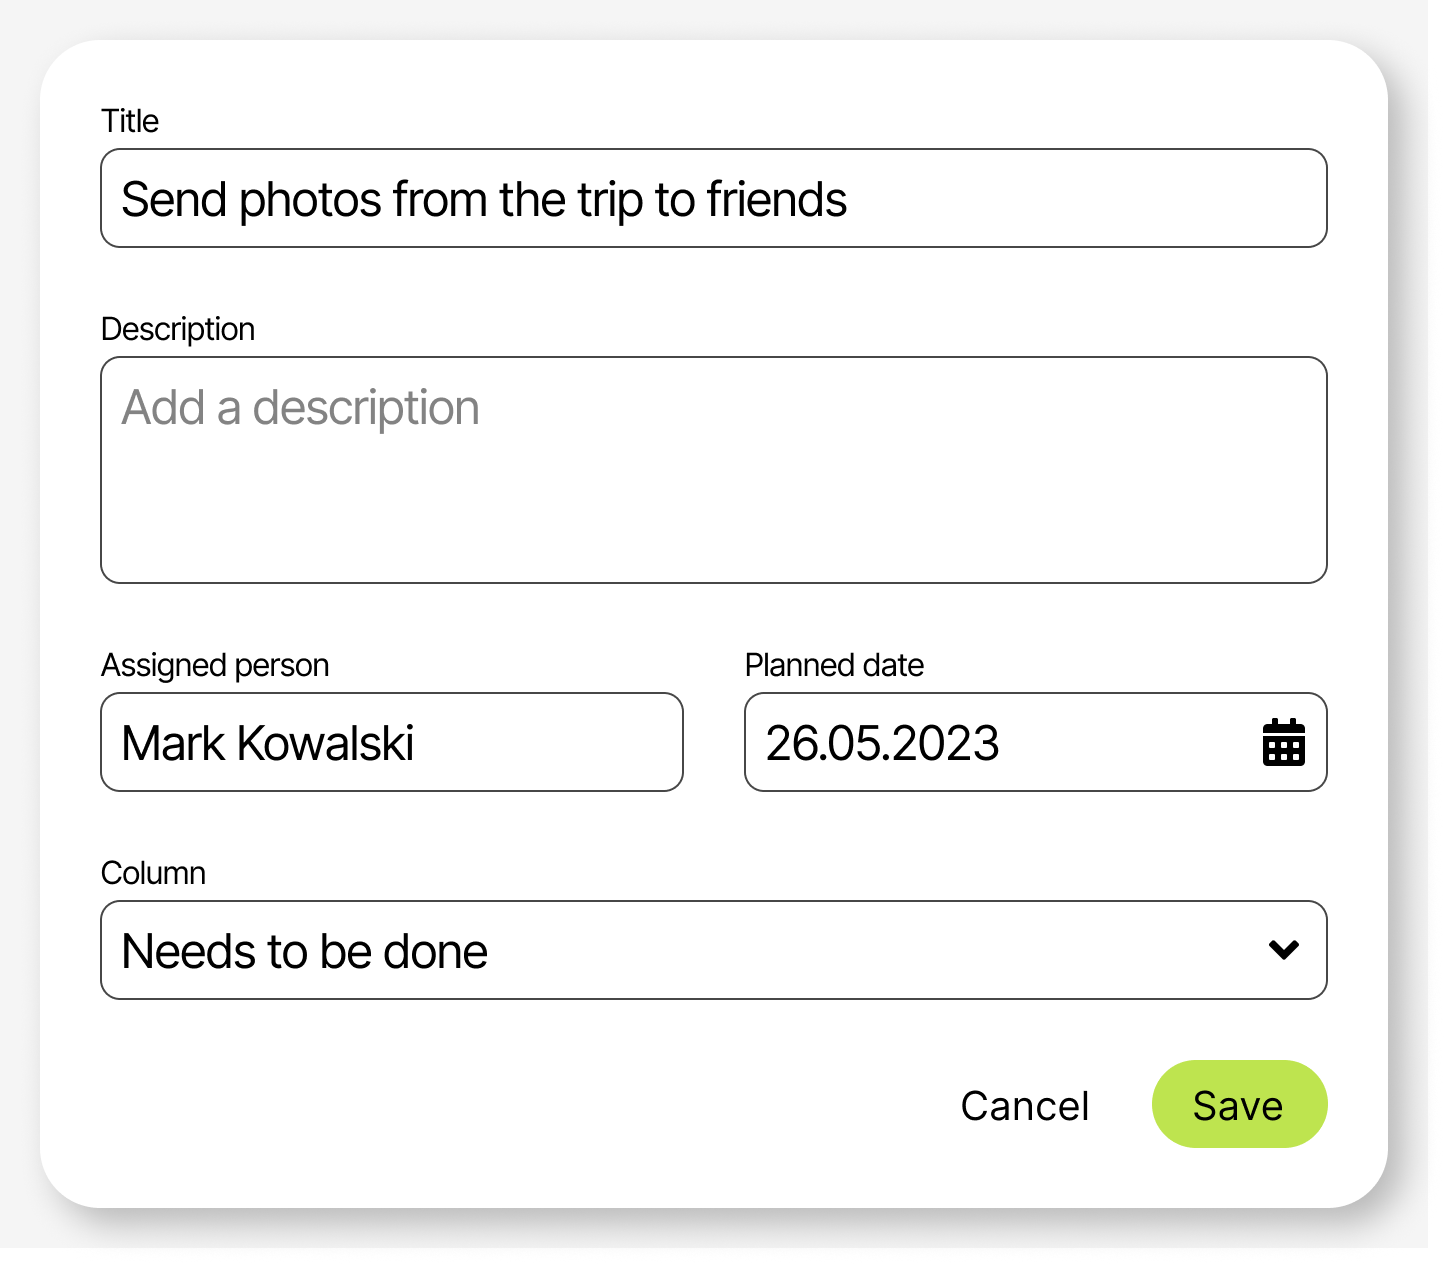
\includegraphics[width=\textwidth]{./3-research-methodology/card-dialog}
        \caption{Card editing dialog in a default state}
        \label{fig:3-4-card-dialog-default}
    \end{subfigure}
    \hfill
    \begin{subfigure}[m]{0.45\textwidth}
        \centering
        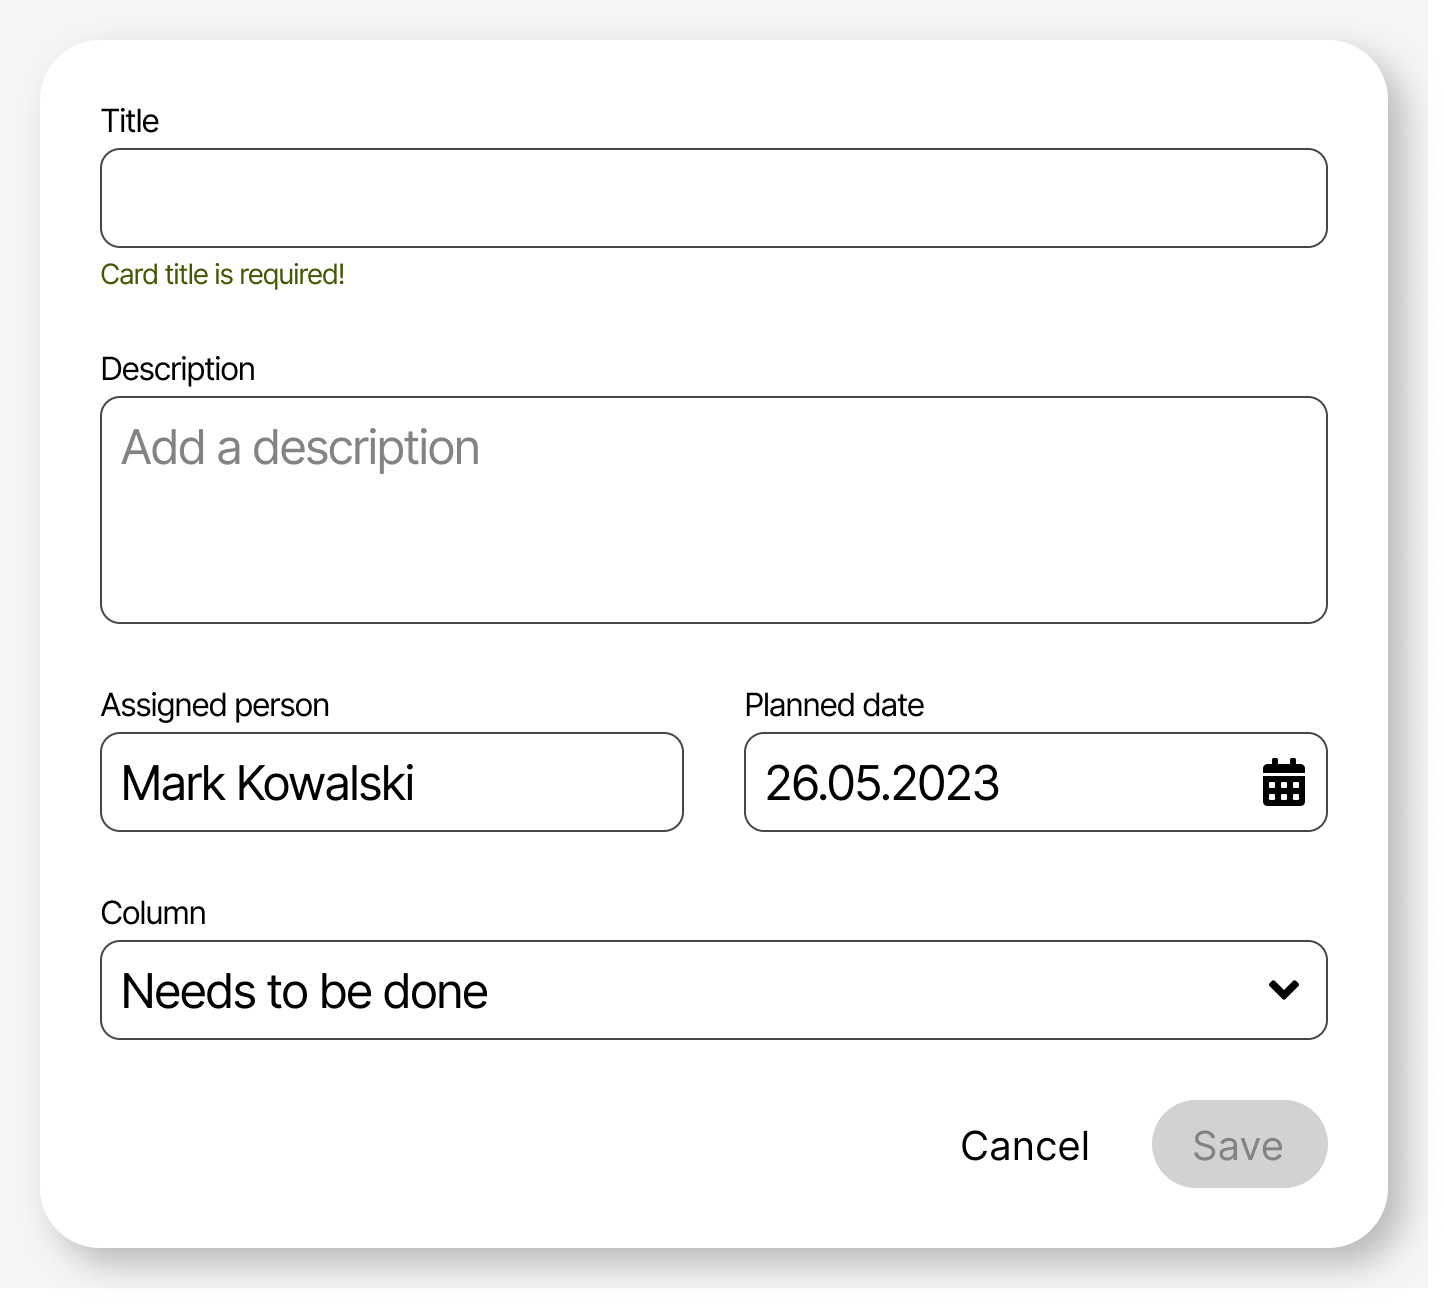
\includegraphics[width=\textwidth]{./3-research-methodology/card-dialog-with-error}
        \caption{Card editing dialog with input error.}
        \label{fig:3-4-card-dialog-with-error}
    \end{subfigure}
    \caption{An example design of a card editing dialog}
    \label{fig:3-4-card-dialog}
\end{figure}

